\documentclass[addpoints]{exam}

\usepackage{amsmath}
\usepackage{amssymb}
\usepackage{graphicx}
\usepackage{hyperref}
\usepackage{multicol}
\usepackage{tikz}
\usepackage{titling}
\usepackage{tabularx}
\usepackage{bookmark}

% Header and footer.
\pagestyle{headandfoot}
\runningheadrule
\runningfootrule
\runningheader{CS 113 Spring 201}{HW 3: Inference and Relations}{\theauthor}
\runningfooter{}{Page \thepage\ of \numpages}{}
\firstpageheader{}{}{}

\boxedpoints
\printanswers

\newcommand\union\cup
\newcommand\interx\cap

\graphicspath{{images/}}

\title{Homework 3: Inference and Relations}
\author{connected-argument}  % replace with your team name
\date{CS/MATH 113 Discrete Mathematics\\Habib University, Spring 2022}

\begin{document}
\maketitle

\begin{questions}

  \section{Inference}
  
\question Prove the following arguments using inference rules. Mention the rule(s) that you use at each step.
  \begin{parts}
    
  \part[5] $ $\\
    \begin{tabular}{ll}
      P1 &  If it is Sunday today, then we play cricket or basketball.\\
      P2 &  If the basketball field is occupied, we don't play basketball.\\
      P3 &  It is Sunday today, and the basketball field is occupied.    \\
      \hline
      C & We play cricket or volleyball. 
    \end{tabular}
    \begin{solution}
      The propositions are as follows: \\
      \begin{tabularx}{\textwidth}{l@{ : }X}
        p & it is Sunday today \\
        q & we play cricket \\ 
        r & we play basketball \\
        s & basketball field is occupied \\
        t & we play volleyball \\
      \end{tabularx}
      \\\\The arguments as propositional logic are as follows: \\
      \begin{tabular}{ll}
        P1 & p $\implies$ $(\text{q} \lor \text{r})$ \\
        P2 & s $\implies \neg$ r \\
        P3 & p $\land$ s \\\hline
        C & q $\lor$ t
      \end{tabular}
      \\\\ Starting from P3: \\
        \begin{tabular}{ll}
          p $ \land $ s \\\hline
          $\therefore$ p & (by Simplification) \\
          $\therefore$ s & (by Simplification)
        \end{tabular}
        \\\\From P1: \\
        \begin{tabular}{ll}
          p $\implies$ (q $\lor$ r) \\\hline
          $\therefore$ q $\lor$ r & (Modus Ponens) 
        \end{tabular}
        \\\\Since p is true, then q or r must be true.
        \\\\From P3: \\
        \begin{tabular}{ll}
          s $ \implies \neg $ r \\\hline
          $\therefore \neg$ r & (Modus Ponens)
        \end{tabular}
        \\\\Since s is true, then negation of r must be true
        \\\\q or r is true, and negation of r is true, then: \\
        \begin{tabular}{ll}
          q $\lor$ r \\
          $\neg$ r \\\hline
          $\therefore$ q & (by Disjunctive Syllogism)\\
        \end{tabular}
        \\\\q is true, then: \\
        \begin{tabular}{ll}
          q \\\hline
          $\therefore$ q $\lor$ t & (by Addition)
        \end{tabular}
        \\Since q is true, then q or t must be true, so it has been proved that the argument is valid. 
    \end{solution}
    
  \part[10]  $ $\\
    \begin{tabular}{ll}
      P1 &  Ahmed failed the course, but attended every lecture. \\
      P2 &  Everyone who did the homework every week passed the course. \\
      P3 &  If a student passed the course, then they did some of the homework.\\
      \hline
      C & Not every student did every homework assignment.
    \end{tabular}

    \begin{solution}
      \\Let S(s) be ``student `s' has passed the course'' \\
      Let LW(s, w) be `` student `s' attended every lecture in week `w' '' \\
      Let HW(s, h) be `` student `s' did every homeowork `h' '' \\
      The Domain for `s' is all students, the domain for `w' is all weeks, the domain for `h' is all homeworks \\\\
      The arguments as Predicate Logic are as follows: \\
      \begin{tabular}{ll}
        P1 & $ \neg P(Ahmed) \land \forall w LW(Ahmed, w) $ \\  
        P2 & $ \forall s \forall h HW(s, h) \implies \forall P(s) $ \\
        P3 & $ \forall s P(s) \implies \exists h HW(s, h) $ \\\hline
        C & $ \exists s \exists h \neg HW(s, h) $ \\
      \end{tabular}
      \\\\ Then: \\ 
      \begin{tabular}{ll}
        1) $ \neg P(Ahmed) \land \forall w LW(Ahmed, w) $ & (P1) \\
        2) $ \neg P(Ahmed) $ & (By Simplification of 1) \\
        3) $ \forall s \forall h HW(s, h) \implies \forall P(s) $ & (P2) \\
        4) $ \forall h HW(Ahmed, h) \implies P(Ahmed) $ & (Universal Instantiation of 3) \\
        5) $ \neg \forall h HW(Ahmed, h) $ & (Modus Tollens on 2 and 4) \\
        6) $ \exists s \neg \forall h HW(s, h) $ & (Existential Generalization of 5) \\
        7) $ \exists s \exists h \neg HW(s, h) $ & (Negating Quantifier of 6) \\
      \end{tabular}
      \\ As shown, we reach the conclusion from the argument, thus the argument is proved to be valid.
    \end{solution}
  \end{parts}

\question[5]
  Consider the statement: The remainder of the square of any odd number when divided by 4 is 1.
  
  \begin{parts}
  \part[5] Write the above statement using predicate logic notation and prove it.
    \begin{solution} 
      \\If k $ \in \mathbb{Z} $ and R(x) is the remainder of the square of x when divided by 4,\\ 
      the given statement can be expressed as:\\
      $ \forall k ((2k+1)^2/4 \to R(2k+1)=1)     \because $ all odd numbers can be expressed as 2k+1 where $ k \in \mathbb{Z} $ \\
      Direct Proof:\\
      Taking antecedent or premise to be true $((2k+1)^2/4)$, we have to prove \\
      that conclusion/consequence (remainder=1) can be expressed in the form of (quotient/dividend + 1). \\
      Here,    $ ((2k+1)^2)/4$ \\
      $ (4k^2 + 4k + 1)/4$ \\
      $ (4k^2/4 + 4k/4 + 1/4 + 1 - 1)$ \\
      $ (4k^2/4 + 4k/4 - 3/4 + 1$ \\
      $ (4k^2 + 4k - 3)/4 + 1$ \\
      where $(4k^2 + 4k - 3)$ is the quotient, 4 is the dividend and 1 is the remainder, as given in the statement. Hence, it is proven that the remainder of the square of any odd number when divided by 4 is 1.

      

    \end{solution}
    
  \part[5] Write the statement from above using a bi-conditional instead of a conditional. Prove whether the new statement holds.
    \begin{solution}
      \\Now considering $((2k+1)^2/4 \Leftrightarrow R(2k+1)=1)$ or \\
      $ ((2k+1)^2/4 \to R(2k+1)=1) \land (R(2k+1)=1 \to (2k+1)^2/4) $\\
      As we have already proven $ ((2k+1)^2/4 \to R(2k+1)=1) $ in part, let's consider $ (R(2k+1)=1 \to (2k+1)^2/4) $\\
      This does not hold as given by a counter example where the remainder is 1, but an odd number is not divided by 4,\\
      Counter example: the remainder of 4/3 is 1, but neither the numerator is odd or divided 4.\\
      Hence, the bioconditional does not hold. 
      odd number
    \end{solution}
  \end{parts}

\question[5]
  Show that these statements about the real number $x$ are equivalent: (i) x is irrational, (ii)  $\frac{x}{2}$ is irrational. Which proof method did you use?

  \begin{solution}
    (Proof by Contradiction) \\
    Suppose that x is irrational, however, $\frac{x}{2}$ is rational. Then $\frac{x}{2}$ can be represented as $\frac{p}{q}$ where p and q
    are integers in their simplest form and q $\neq$ 0. So $\frac{x}{2} = \frac{p}{q}$. Then $x = \frac{2p}{q}$. Since $2p$ is also an integer,
    let $2p = r$. Then $x = \frac{r}{q}$. But x is irrational and cannot be represented in the form of $\frac{a}{b}$ thus we have a contradiction.
    So $\frac{x}{2}$ must be irrational. Moreover, the same can be argued when $\frac{x}{2}$ is supposed to be irrational and $x$ is supposed to be rational. 
    As $x$ is rational, it can be represented as $\frac{p}{q}$ where p and q are integers in their simplest form and q $\neq$ 0. Then $x = \frac{p}{q}$.
    Dividing both sides by $2$ results in $\frac{x}{2} = \frac{p}{2q}$. However, since $\frac{x}{2}$ is irratinoal, it cannot be represented as $\frac{a}{b}$. Thus 
    we have a contradiction. Hence proved that the two statements are equivalent. 
  \end{solution}

\question This question refers to the \textit{tiling} or \href{https://en.wikipedia.org/wiki/Tessellation}{\textit{tessellation}} operation.
  
  \begin{minipage}{0.5 \linewidth}
    Given a standard checkerboard and dominoes, answer the following questions. Explain your answer for each question.
    \begin{center}
      \includegraphics[width= 0.15\textwidth]{dominos}
    \end{center}
  \end{minipage} 
  \begin{minipage}{0.5 \linewidth}\begin{center}
      \includegraphics[width=0.6 \textwidth]{checkerboard} \end{center}
  \end{minipage}
  \begin{parts}
  \part[5] Can we tile the standard checkerboard using dominoes?
    \begin{solution}\\
      Yes, we can tile a standard 8x8 checkerboard dominoes. Since a domino has the size of two checkerboard boxes and a checkerboard is contains 64 total boxes. Then it can be tiled by 32 dominoes, placing the dominoes parallel to eachother.
    \end{solution}
    
  \part[5] Can we tile a checkerboard obtained by removing one of the four corner squares of a standard checkerboard?
    \begin{solution}\\
      No, a checkerboard cannot be tiled by removing one of the corners. If a corner is removed. The number of boxes are not even anymore and cannot be tiled with 1x2 size dominoes. \\
      Proof by contradiction:\\
      Suppose one of the four corners is removed from the checkerboard and we are left with 63 boxes instead of 64. In this case if we want to tile the checkerboard using dominoes, one tile will always be extra and left in the checkerboard. This results in contradiction and we must not remove any corners of the checkerboardin order to tile it dominoes. 

    \end{solution}
    
  \part[5] Can we tile a board obtained by removing both the upper left and the lower right squares of a standard checkerboard? 
    \begin{solution}
      \\Proof by contradiction:\\
      Let's suppose the board has upper left and lower right squares removed. Now in order to tile this board we need 31 dominoes. Since a domino has one black and one white tile. So we will have equal numbers of black and white tiles on the board. However, the oriantaion of the checkerboardis such that opposite ends have same colored tiles. So if we removed opposite white squares, the dominoes should be able to account for 30 white tiles and 32 black tiles. Since each domino only has two tiles, this cannot be achieved and contradiction arises. 
      Hence, our assumption was wrong and the checkerboard cannot be tiled if the upper left and the lower right squares are removed.
       
    \end{solution}
  \end{parts}

\question[10]
  The following is a murder case solved by Sherlock Holmes, in “A Study
  in Scarlet” :\\
  \textit{“And now we come to the great question as to the reason why. Robbery
    has not been the object of the murder, for nothing was taken. Was it
    politics, then, or was it a woman?  That is the question which confronted
    me. I was inclined from the first to the latter supposition. Political
    assassins are only too glad to do their work and fly. This murder had, on
    the contrary, been done most deliberately, and the perpetrator has left
    his tracks all over the room, showing he had been
    there all the time.”}\\
  From these, Sherlock Holmes concluded: ``It was a woman''.  Translate the
  above argument to statements in predicate logic and prove its validity.
  \begin{solution}
    The simple propositions are as follows: \\
    \begin{tabularx}{\textwidth}{l@{ : }X}
      p & it's a robbery \\
      q & something was taken \\
      r & the object of murder involved politics \\
      s & a woman was involved \\
      t & assassin left as soon as the work was finished \\
      u & assassin left tracks
    \end{tabularx}
    The arguments can be written as follows: \\
    \begin{tabularx}{\textwidth}{l@{ : }X}
      P1 & if it's a robbery, then something was taken \\
      P2 & nothing was taken \\ 
      P3 & if it's not a robbery, then it was either politics or a woman \\
      P4 & if it's politics, then the assassin would have left as soon as the work was finished \\
      P5 & if the assassin left tracks, then he did not leave as soon as the work was finished \\
      P6 & the assassin left tracks \\
    \end{tabularx}
    The situation can then be represented as follows: \\
    \begin{tabularx}{\textwidth}{l@{ : }X}
      1 & p $\implies$ q \\
      2 & $\neg$ q \\
      3 & $ \neg p \implies (r \lor s) $ \\
      4 & $ r \implies t$ \\
      5 & $ u \implies \neg t$ \\
      6 & u
    \end{tabularx}
    From P2: \\
    $\neg$ q \\
    From P1 and P2: \\
    \begin{tabular}{ll}
      $ \neg $ q \\
      $ p \implies q $ \\\hline
      $ \therefore \neg p $ & (by Modus Tollens)
    \end{tabular}
    \\ Thus it was not a robbery. \\
    From P3: \\
    \begin{tabular}{ll}
      $ \neg p $ \\\hline
      $ r \lor s $ & (By Addition)
    \end{tabular}
    \\ So it was either due to politics, or a woman was involved. \\
    From P6: \\
    u \\
    From P5 and P6: \\
    \begin{tabular}{ll}
      u \\
      $ u \implies \neg t$ \\\hline
      $ \therefore \neg t $ & (by Modus Ponens)
    \end{tabular}
    \\ Since the assassin left tracks, the assassin did not leave as soon as the work was finished. \\
    Then: \\
    \begin{tabular}{ll}
      $\neg t$ \\
      $r \implies t$ \\\hline
      $ \therefore \neg r$ & (by Modus Tonens)
    \end{tabular}
    \\ Then the object of murder did not involve politics.\\
    Therefore: \\
    \begin{tabular}{ll}
      $r \lor s$ \\
      $\neg r$ \\\hline
      $ \therefore s $ & (by Disjunctive Syllogism)
    \end{tabular}
    \\Hence we prove that the argument is valid and a woman was involved.
  \end{solution}
  
  \section{Equivalence Relation}
  
\question Prove or disprove whether each of the relations represented below is an equivalence relation.
  \begin{parts}
  \part[5] $R \text{ on } \mathbb{R} = \{ (x,y) \mid xy\geq 0\}$
  \part[5] $R \text{ on } \mathbb{R} = \{ (x,y) \mid x = 1\}$
  \part[5] $\begin{bmatrix} 1 & 0 & 1 & 0 \\ 0 & 1 & 0 & 1 \\1 & 0 & 1 & 0 \\ 0 & 1 & 0 & 1 \end{bmatrix}$
  \part[5] $\begin{bmatrix} 1 & 1 & 1 & 0 \\ 1 & 1 & 1 & 0 \\ 1 & 1 & 1 & 0 \\ 0 & 0 & 0 & 1 \end{bmatrix}$
  \part[5] $R_1 \interx R_2$ where $R_1$ and $R_2$ are equivalence relations on a set, $S$.
  \end{parts}
  \begin{solution}
    % Write your solutions here
    \begin{parts}
      \part
        Three properties for equivalence: 1. Reflexivity 2. Symmetry 3. Transitivity\\
        $ \mathbb{R} = \{ (x,y) \mid xy\geq 0\}$ \\
        1. Reflexivity: $\forall a \in \mathbb{R} \to (a,a) \in R $\\ 
        As squares of numbers are always positive, i.e. $x^2$, $y^2$ 
        hence if (x,y) $\in R$ then (x,x) $\in R$ and (y,y) $\in R$\\
        2. Symmetry: Since multiplicaion is a commutative operatione i.e. the order of operation does not matter, this relation is symmetric, expressed as:\\
        $(x,y) \in R \to (y,x) \in R$\\
        3. Transitivity: By definition $ xy\geq 0 $ R contains every positive elements of first set to the positive elements of second set and negative elements of first set and negative elements of second set.\\
        Hence, lets suppose $xRy$ and $yRc$. Either x, y , and z will be positive or negative. So if all are postive, \\
        $xRc \because xy \geq 0$ and if all are negative, $ xRy \land yRc \to xRc \because (-x)*(-c) = xc \geq 0 xc\geq 0 $ \\
    \part\
    $R \text{ on } \mathbb{R} = \{ (x,y) \mid x = 1\}$
    1. Reflexivity: $\forall a \in \mathbb{R} \to (a,a) \in R $\\ 
    Here, x is a constant that is not changing and at every value of y, x remains the same. Hence, this relation is not relfexive.
    Counterexample:
    (1,0), given the definition of reflexivity, both (1,1) and (0,0) $\in R$. However, the value of x is always 1 and nothing else. Hence, the relation is not reflexive.
    2. Symmetry: $(x,y) \in R \to (y,x) \in R$\\
    Since x is constant, no matter how much y changes, x will remain 1.\\
    Counterexample: (1,0) $\in R $ but not (0,1) $\in R $ \\
    3. Transitivity: $unsure$
    \part
    1. Reflexivity: $\forall a \in \mathbb{R} \to (a,a) \in R $\\ 
    Here, the diagonal suggests that the relation is indeed reflexive. Let the rows of be i and columns be j. We see that for all i's and j's positions where i=j there exists 1 in the graph which indicates that the aRa for all values in the relation. Hence, it proved that the relation is reflexive.
    2. Symmetry: $(x,y) \in R \to (y,x) \in R$\\
    Symmetry of a relation through graphical representation is expressed as same elements on the non diagonals, i.e. if position ij = 0 then ji = 0 or if ij = 1 then ji = 1, this proves that the relation is  indeed symmetric.
    3. Transitivity: if $(x,y) \in R \land (y,z) \in R \to (x,z) \in R$ \\
    To observe the matrix, let's call the rows and columns 1,2,3,4. Now for transitivity,\\
    $ (0,3) \land (3,0) \to (0,0)$\\
    $ (2,1) \land (1,4) \to (2,4)$\\
    \dots
    $ (4,2) \land (2,4) \to (4,4)$\\
    There are no counterexamples, hence, transitivity is proven\\    
    \part
    1. Reflexivity: $\forall a \in \mathbb{R} \to (a,a) \in R $\\ 
    Here, the diagonal suggests that the relation is indeed reflexive. Let the rows of be i and columns be j. We see that for all i's and j's positions where i=j there exists 1 in the graph which indicates that the aRa for all values in the relation. Hence, it proved that the relation is reflexive.
    2. Symmetry: $(x,y) \in R \to (y,x) \in R$\\
    Symmetry of a relation through graphical representation is expressed as same elements on the non diagonals, i.e. if position ij = 0 then ji = 0 or if ij = 1 then ji = 1, this proves that the relation is  indeed symmetric.
    3. Transitivity: if $(x,y) \in R \land (y,z) \in R \to (x,z) \in R$ \\
    To observe the matrix, let's again call the rows and columns 1,2,3,4. Now for transitivity,\\
    $ (1,2) \land (2,3) \to (1,3)$\\
    $ (2,3) \land (3,1) \to (2,1)$\\
    \dots
    $ (4,4) \land (4,4) \to (4,4)$\\
    There are no counterexamples, hence, transitivity is proven\\
    \part
      tbd
    
    \end{parts}    
  \end{solution}

  \begin{EnvUplevel}
    Let $R$ be a relation from a set A to a set B. The \textit{inverse relation} from $B$ to $A$, denoted by $R^{-1}$, is the set of ordered pairs $\{(b, a) \mid (a, b) \in R\}$. The \textit{complementary relation} $\overline{R}$ is the set of ordered pairs $\{(a, b) \mid (a, b) \not\in R\}$. A relation $R$ on the set $A$ is \textit{irreflexive} if $\forall a \in A\colon (a, a) \not\in R$. That is, $R$ is irreflexive if no element in $A$ is related to itself.
  \end{EnvUplevel}

\question 
  \begin{parts}
  \part[5] Show that the relation $R$ on a set $A$ is symmetric if and only if $R = R^{-1}$.
    \begin{solution}
      If $R = R^{-1}$, then $R \subseteq R^{-1}$ and $R^{-1} \subseteq R$.\\
      \underline{\textbf{If} $R = R^{-1}$:} If $R$ is symmetric, then $\forall a,b \in A$, $(a, b) \in R \text{ and } (b, a) \in R \text{, so } (a, b) \in R^{-1}$ (by definition of inverse of relation). Thus, $R \subseteq R^{-1}$. Moreover, $R^{-1} \subseteq R$. Therefore, $R = R^{-1}$
      \underline{\textbf{Only If} $R = R^{-1}$:} Conversely, if $R = R^{-1}$ and $(a, b) \in R \text{, then } (b, a) \in R^{-1} \text{, so } (b, a) \in R$. Thus $R$ is symmetric. 
    \end{solution}

  \part[5] Show that the relation $R$ on a set $A$ is reflexive if and only if $\overline{R}$ is irreflexive.
    \begin{solution}
      By the definition of the complementary relation $\overline{R} \text{, if } (a, b) \notin R, (a, b) \in \overline{R}$. $R$ is reflexive if and only if $R$ contains all the pairs $(a, a)$. Then by definition of complementary relation, none of those pairs can exist in $\overline{R}$. Thus the pairs $(a, a) \notin R$, then by definition of irreflexive, $\overline{R}$ is irreflexive. So $R$ can only be reflexive if its complementary relation $\overline{R}$ is irreflexive. Hence proved.
    \end{solution}

  \part[5] Let $R$ be a relation that is reflexive and transitive. Prove that $R^n = R$ for all positive integers $n$.
    \begin{solution}
      (Proof by Induction) \\
      $R^{n} = R$, by definition of composite relations, $R^{n} = R^{n-1} \circ R$. Thus $R^{n-1} \circ R \subseteq R \text{, and } R \subseteq R^{n-1} \circ R$ \\
      \underline{\textbf{For Reflexive:}} \\
      \textbf{Base Step (n = 1):} $R^{1} = R$ (Trivial Proof). R is reflexive \\
      \textbf{Assumption (n = k):} Assume that $R^{k}$ is reflexive. Then for all pairs, $(a, a) \in R$ and $(a, a) \in R^{k}$. \\
      \textbf{Inductive Step (n = k+1):} By definitin, $R^{k+1} = R^{k} \circ R$. Since for all pairs $(a, a) \in R$, and $(a, a) \in R^{k}$, so $(a, a) \in R^{k + 1}$. \\\\
      
      \underline{\textbf{For Transitive:}} \\
      \textbf{Base Step, (n = 1):} $R^{1} = R$ (Trivial Proof). R is transitive. \\
      \textbf{Assumption, (n = k):} Assume that $R^{k}$ is transitive. So our inductive hypothesis becomes that $R^{k} = R$ \\
      \textbf{Inductive Step, (n = k + 1):} By definition, $R^{k+1} = R^{k} \circ R$. For a pair $(a, c) \in R^{n} \circ R$, there must exist an element $b$ such that $(a, b) \in R \text{, and } (b, c) \in R^{k}$. Then by the inductive hypothesis, $(b, c) \in R$. Since $R$ is transitive, $(a, c) \in R$, and also since $R^{k} = R$, $(a, b) \in R^{k}$ so $(a, c) \in R^{k}$. \\
      So it can be concluded from above that $R^{n} \subseteq R$ and $R \subseteq R^{n}$. Thus proved that $R^{n} = R$ where R is a relation that is reflexive and transitive.
    \end{solution}

  \part[5] Show that the relation $R$ on a set $A$ is transitive if and only if $R^n \subseteq R$ for all positive integers $n$.
    \begin{solution}
      \textbf{If:} Suppose that $R^{n} \subseteq R$ for n = 2 (trivial for n = 1). Then $R^{2} \subseteq R$. If $(a, b) \in R$, and $(b, c) \in R$ then by definition of composite relation, $(a, c) \in R^{2}$. Since $R^{2} \subseteq R$, then $(a, c) \in R$ as well. Hence $R$ is transitive. \\
      \textbf{Only if:} (Proof by induction) \\
      Statement is trivially true for n = 1. $R^{1} \subseteq R$ \\
      Assume that $R^{n} \subseteq R$. Then $R^{n+1}$ must also be a subset of $R$. By definition, $R^{n+1} = R^{n} \circ R$. Assume that $(a, c) \in R^{n+1}$, then there is an element $b$ such that $(a, b) \in R$ and $(b, c) \in R^{n}$. Then $R^{n} \subseteq R$ implies that $(b, c) \in R$. Also since $R$ is transitive, $(a, c) \in R$ since $(a, b) \in R$ and $(b, c) \in R$. Since $(a, c) \in R$ and $(a, c) \in R^{n+1}$, this shows that $R^{n+1} \subseteq R$. Hence proved. 
    \end{solution}

  \end{parts}
  
\question  Given the matrix, $M_R$, for a relation, $R$, on a finite set, $A$, explain how to obtain the following matrices?
  \begin{multicols}{2}
    \begin{parts}
    \part[5] $M_{R^{-1}}$
    \part[5] $M_{\overline{R}}$
    \end{parts}
  \end{multicols}
  \begin{solution}
    % Write your solutions here
    \begin{parts}
    \part 
      We know that $M_{R^{-1}}$ is defined as $M_{R^{-1}} = \{(b,a) \mid (a,b) \in R\}$\\
      In other words, the order of the ordered pairs in the relation is reversed. In terms of matrix representation, it can be expressed as a transpose of the original matrix ${M}$.\\
      The transpose of a matrix is obtained by swapping the rows and and columns of the matrix. So, the values that were represented by the columns would now be represented by rows and vice versa. This obtains the desired matrix representation for $M_{R^{-1}}$.
    \part 
      $M_{\overline{R}}$ is defined as the complementary relation over M: $M_{\overline{R}} = \{(a,b) \mid (a,b) \notin R\}$\\
      Here the matrix representation swaps 1's and 0's. To represent that (a,b) exists in the relation M, $M_ij$ = 1 for the respective row (i) and column (j). However to represent $M_{\overline{R}}$, instead of 1 the ${M_{\overline{R}}}_{ij}$ = 0 indicating the absence of (a,b) $\in R$ in $M_{\overline{R}}$.
 
      
      
    \end{parts}
  \end{solution}
  
\question The following questions refer to the relations, $R$ and $S$, involving the set $X = \{a, b, c\}$. Specifically, $R$ and $S$ are relations on $2^X$, the power set of $X$. For the definitions of $R$ and $S$ given below, prove whether each is an equivalence relation.
  \begin{multicols}{2}
    \begin{parts}
    \part[5] $R = \{(A, B) \mid |A| = |B|\}$.
    \part[5] $S = \{(A, B) \mid |A| < |B|\}$.
    \end{parts}
  \end{multicols}
  \begin{solution}
    % Write your solutions here
    \begin{parts}
    \part R will be reflexive as for any element $A \in 2^X$, the cardinality of A is equal to itself. Therefore, $(A, A) \in R$. 
    R will also be symmetric as for $A, B \in 2^X$, if $|A|$ is equal to $|B|$, then $|B|$ is also equal to $|A|$. Therefore, $(A, B) \in R$, and $(B, A) \in R$ as well. 
    R will be transitive as for $A, B, C \in 2^X$. If $|A|$ is equal to $|B|$, and $|B|$ is equal to $|C|$, then $|A|$ is also equal to $|C|$. Thus R will be transitive. \\
    Since R is reflexive, symmetric and transitive, R is an equivalence relation.
    \part S will not be reflexive as for any element $A \in 2^X$, the cardinality of that element cannot be less than itself. Thus S will not be reflexive. 
    Moreover, S is also not symmetric as for $A, B \in 2^X$, if $|A| < |B|$, then $|B| \nless |A|$, therefore S is also not symmetric. So it can be concluded that S is not an equivalence relation.
    \end{parts}
  \end{solution}

\question[5] A partition $P_1$ is called a \textit{refinement} of the partition $P_2$ if every set in $P_1$ is a subset of one of the sets in $P_2$. Given equivalence relations, $R_1$ and $R_2$, on a set, $A$, and the corresponding partitions, $P_1$ and $P_2$, show that $R_1 \subseteq R_2$ if and only if $P_1$ is a refinement of $P_2$.
  \begin{solution}
    \\ $P_1$ is a refinement of $P_2$ can be expressed as:\\
    $ \forall a \exists b  (a \subseteq b) | (a \in P_1) (b \in P_2)$\\
    since partitions $P_1$ and $P_2$ correspond to relations $R_1$ and $R_2$ on set A respectively, above statement can also be written as,
    \\$ \forall a \exists b  (a \subseteq b) | (a \in xR_1y) (b \in xR_2y)$\\
    To show that  $R_1 \subseteq R_2 \iff \forall a \exists b  (a \subseteq b) | (a \in xR_1y) (b \in xR_2y)$\\
    First $R_1 \subseteq R_2 \Rightarrow \forall a \exists b  (a \subseteq b) | (a \in xR_1y) (b \in xR_2y)$\\
    Let $|a|$ be a representative of a random equivalence class in $R_1$ on set A then as per the definition of a class, every element of this class exists in $xR_1y$ or $|a|_{R_1} \subseteq xR_1y$ for a random class $|a|_{R_1}$ in $R_1$.\\
    We know that $R_1 \subseteq R_2$, through transivity we can say that $|a|_{R_1} \subseteq R_2$ \\
    Since $|a|R_1$ was a random equivalence class, this can be generalized for all the equivalence classes of $R_1$:\\
    $\forall a : |a|_{R_1}  (|a|_{R_1} \subseteq R_2$)
    \\Like we did for $R_1$ we can deduce that every equivalence class in $R_2$ is a subset of $R_2$:
    \\$\forall b : |b|_{R_2}  (|b|_{R_2} \subseteq R_2$)
    \\$R_2$ can also be written as the union of all partitions of $R_2$
    \\$\forall b : |b|_{R_2} (|b|_{R_2} \subseteq U_{Pi_{R_2}})$ where $U_{Pi_{R_2}}$ represents the union of all the equivalent classes of $R_2.$\\
    By the definition of a union then we can conclude that $|a|R_1$ is the subset of at least one partition of $R_2$ and hence:\\
    $\forall a :  |a|_{R_1} \exists P_2 : P_2 \in R_2 (|a|_{R_1} \subseteq P_2)$
    By using the transitivity property of subsets, let $b \subseteq P_2$
    $\forall a \exists b (|a|_{R_1} \subseteq P_2) | (|a|_{R_1}) (b \in P_2) $\\
    It is the same definition as $P_1$ is a refinement of $P_2$. Hence proven that \\
    $R_1 \subseteq R_2 \Rightarrow \forall a \exists b  (a \subseteq b) | (a \in xR_1y) (b \in xR_2y)$\\
    Following the same method $\forall a \exists b  (a \subseteq b) | (a \in xR_1y) (b \in xR_2y) \Rightarrow R_1 \subseteq R_2$ can also be proved.\\


  \end{solution}

  \section{Ordering}
  
\question Prove or disprove whether each of the relations represented below is a partial order.
  \begin{multicols}{3}
    \begin{parts}
    \part[5] $\begin{bmatrix} 1 & 1 & 1 \\ 1 & 1 & 0 \\ 0 & 0 & 1 \end{bmatrix}$
    \part[5] $\begin{bmatrix} 1 & 1 & 1 & 0 \\ 1 & 1 & 1 & 0 \\ 0 & 0 & 1 & 1 \\ 1 & 1 & 0 & 1 \end{bmatrix}$
    \end{parts}
  \end{multicols}
  \begin{solution}
    % Write your solutions here
    \begin{parts}
    \part The matrix representing the relation is not antisymmetric since (1, 2) and (2, 1) both exist within the relation, however, 1 $ \neq $ 2. Thus it is not partial order relation.
    \part The matrix representing the relation is not antisymmetric since (1, 2) and (2, 1) both exist within the relation, however, 1 $ \neq $ 2. Moreover, (2, 3) exist, and (3, 4) exists, however, (2, 4) does not exist so it is also not transitive. Thus this relation is not partial order.
    \end{parts}
  \end{solution}
  
\question[5] Given a poset $(S, R)$, its \textit{dual} is $(S,R^{-1})$. Show that the dual is also a poset. 
  \begin{solution}\\
    The inserve relation $R^-1$ is defined as $R^{-1} = \{(b,a) \mid (a,b) \in R\}$\\
    Since (S,R) is a poset then it satisifies, reflextiviy, antisymmetry, and transitivity. \\
    Considering $(S,R^{-1})$:\\
    For reflexivity:
    \\Let a be a random such that (a,a) $\in (S,R)$, since (a,a) is commutative, (a,a) $\in (S,R^{-1})$\\
    Since a is random, it can generalized to all a in $(S,R^{-1})$, hence $(S,R^{-1})$ is reflexive.
    \\For antisymmetry:
    \\Let a random (x,y) $\in (S,R)$, then (x,y) $\in (S,R^{-1})$. Because of the antisymmetry of (S,R), (y,x) does not exist in (S,R) which means (x,y) cannot exist in $(S,R^{-1})$.
    \\This is true for all x,y such that (x,y) and $x \neq y$. Hence, $(S,R^{-1})$ is antisymmetric.
    \\For transitivity:
    \\Let (x,y) $\in (S,R)$ and (y,z) $\in (S,R)$, then as per transitivity (x,c) $\in (S,R)$. Considering the same elements. $(x,y) \in (S,R) \Rightarrow (y,x) \in (S,R^{-1}) \land (y,z) \in (S,R) \Rightarrow (z,y) \in (S,R^{-1})$.
    \\Here, (z,y) and (y,x) indicates that $(z,x) \in (S,R^{-1})$. This is true for all x,y,z such that $(x,y) \in (R,S) \land (y,z) \in (R,S) $  .    
  \end{solution}
  
\question Answer the following questions for the partial order represented by the given Hasse diagram.
  
  \begin{minipage}{.3\textwidth}
    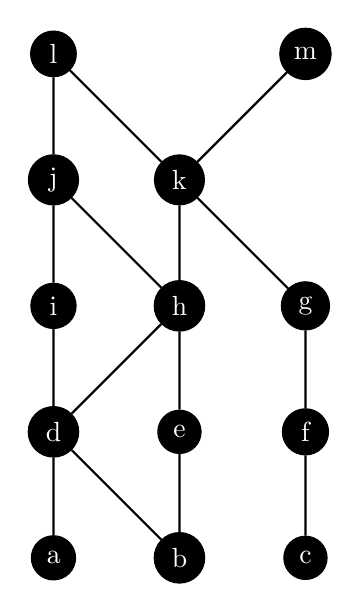
\begin{tikzpicture}[scale=0.8]
      \tikzstyle{node} = [draw,circle,fill=black,text=white]

      \def\nodes{a,b,c,d,e,f,i,h,g,j,k}
      \foreach \n/\p
      [count=\i from 0,
      evaluate= \i as \x using {2*Mod(\i,3)},
      evaluate= \i as \y using {2*int(\i/3)}]
      in \nodes {
        \node[node](\n) at (\x,\y) {\n};
      }
      \node[node](l) at (0,8) {l};
      \node[node](m) at (4,8) {m};

      \draw[thick,-] (a) -- (d) -- (i) -- (j) -- (h) -- (d) -- (b) -- (e) -- (h) -- (k) -- (l) -- (j);
      \draw[thick,-] (c) -- (f) -- (g) -- (k) -- (m);
      
    \end{tikzpicture}
  \end{minipage}
  \begin{minipage}{.65\textwidth}
    \begin{parts}
    \part[2] Find the maximal elements.
    \part[2] Find the minimal elements.
    \part[1] Is there a greatest element? If so, what is it?
    \part[1] Is there a least element? If so, what is it?
    \part[2] Find all upper bounds of $\{a,b,c\}$.
    \part[1] Find the least upper bound of $\{a,b,c\}$, if it exists.
    \part[2] Find all lower bounds of $\{f,g,h\}$.
    \part[1] Find the greatest lower bound of $\{f,g,h\}$, if it exists.
    \end{parts}
  \end{minipage}
  \begin{solution}
    % Write your solutions here
    \begin{parts}
    \part Maximal elements do not have any element above them, so they are $l$ and $m$.
    \part Minimal elements do not have any element below them, so they are $a$, $b$ and $c$. 
    \part A greatest element is a unique element greater than all other elements. $l$ and $m$ are both at the same level, neither is greater, so there is no greatest element.
    \part A least element is a unique element lesser than all other elements. $a$, $b$ and $c$ are both at the same level with none below any other, so there is no least element.
    \part Upper bounds of elements $\{a, b, c\}$ will be common elements from which a downward path can be created to all three elements. Thus the upper bounds will be $l$, $m$ and $k$.
    \part Least upper bound will be the element lesser than all the other upper bounds of $\{a, b, c\}$. $k$ is the least upper bound.
    \part Lower bounds of elements $\{f, g, h\}$ will be common elements from which an upward path can be created to all three elements. However, there is no such common element between $f$ and $h$ thus there are no lower bounds.
    \part There is no greatest lower bound since there are no lower bounds. 
    \end{parts}
  \end{solution}
  
\end{questions}

\end{document}

%%% Local Variables:
%%% mode: latex
%%% TeX-master: t
%%% End:
